% Create a Table of Contents in Beamer
\documentclass[10pt,t]{beamer}
% Theme choice:
\usetheme{Singapore}
\useoutertheme{sidebar}
\usecolortheme{seahorse}
\setbeamercolor{titlelike}{bg=white}
\setbeamercolor{frametitle}{bg=white}
%\setbeamertemplate{frametitle}[default][left]
\setbeamertemplate{navigation symbols}{}

\usepackage{graphicx}
\usepackage{amsmath}
\usepackage{amsfonts}
\usepackage{amssymb}
\usepackage{amsthm}
\usepackage{ulem}
\usepackage{listings}

% Title page details: 
\title{Chapter 1b: Multiple Linear Regression} 
\author{Taylor Okonek \& Charlie Wolock}
\date{\today}


\begin{document}
	% Title page frame
	\begin{frame}
	\titlepage 
\end{frame}

\begin{frame}{Learning objectives}
By the end of Chapter 1b, you should be able to:
\begin{itemize}
	\item Formulate a regression model, given a scientific or statistical question
	\item Interpret the coefficients for a multiple linear regression model
	\item Interpret confidence intervals and p-values for multiple linear regression coefficients
	\item Classify variables according to their role in a linear regression model (e.g., outcome, predictor, potential confounder, effect modifier, precision variable)
	\item Describe why you would adjust for certain variables in a regression analysis
	\item Use \texttt{R} to fit a multiple linear regression model (and know where in the output to look for the information we need to interpret results)
	\item Create graphs to support your linear regression analysis
\end{itemize}
\end{frame}

% Outline frame
\begin{frame}{Outline}
\tableofcontents
\end{frame}

\AtBeginSection[ ]
{
\begin{frame}{Outline}
\tableofcontents[currentsection]
\end{frame}
}

% Presentation structure


\section{Motivation}

\subsection{Linear regression models with multi-level categorical predictors}

\begin{frame}{Linear regression with a categorical predictor}
So far we've seen examples of simple linear regression with a binary predictor. What if instead our scientific question is about the association between a continuous outcome and a \textit{multilevel} (more than two groups) categorical predictor? \pause

\vspace{0.3cm}

If the predictor is binary (e.g. has a genetic variant vs. does not):
\begin{itemize}
	\item Simple linear regression or t-test comparing difference in means between two groups
\end{itemize} \pause

\vspace{0.3cm}

If the predictor is ordinal (e.g. education level: high school, college, masters, etc.):
\begin{itemize}
	\item You \textit{may} be able to find a meaningful way to represent categories numerically (i.e. assign numbers 1 through $k$ to each of $k$ groups)
\end{itemize} \pause

\vspace{0.3cm}

If the predictor is nominal (e.g., country)
\begin{itemize}
	\item No meaningul numeric representation
\end{itemize}

\end{frame}

\begin{frame}{Linear regression with a categorical predictor}
What can we do? \pause We can use \textcolor{blue}{dummy variables}\dots

\vspace{0.3cm}

\textcolor{blue}{Dummy variables}: The set of \textit{binary} variables created by re-writing (or re-coding) a multilevel categorical variable  \pause

\vspace{0.3cm}

Example: Suppose we have a multilevel categorical variable for US region, with values West, Midwest, South, and Northeast

\vspace{0.1cm}

\centering

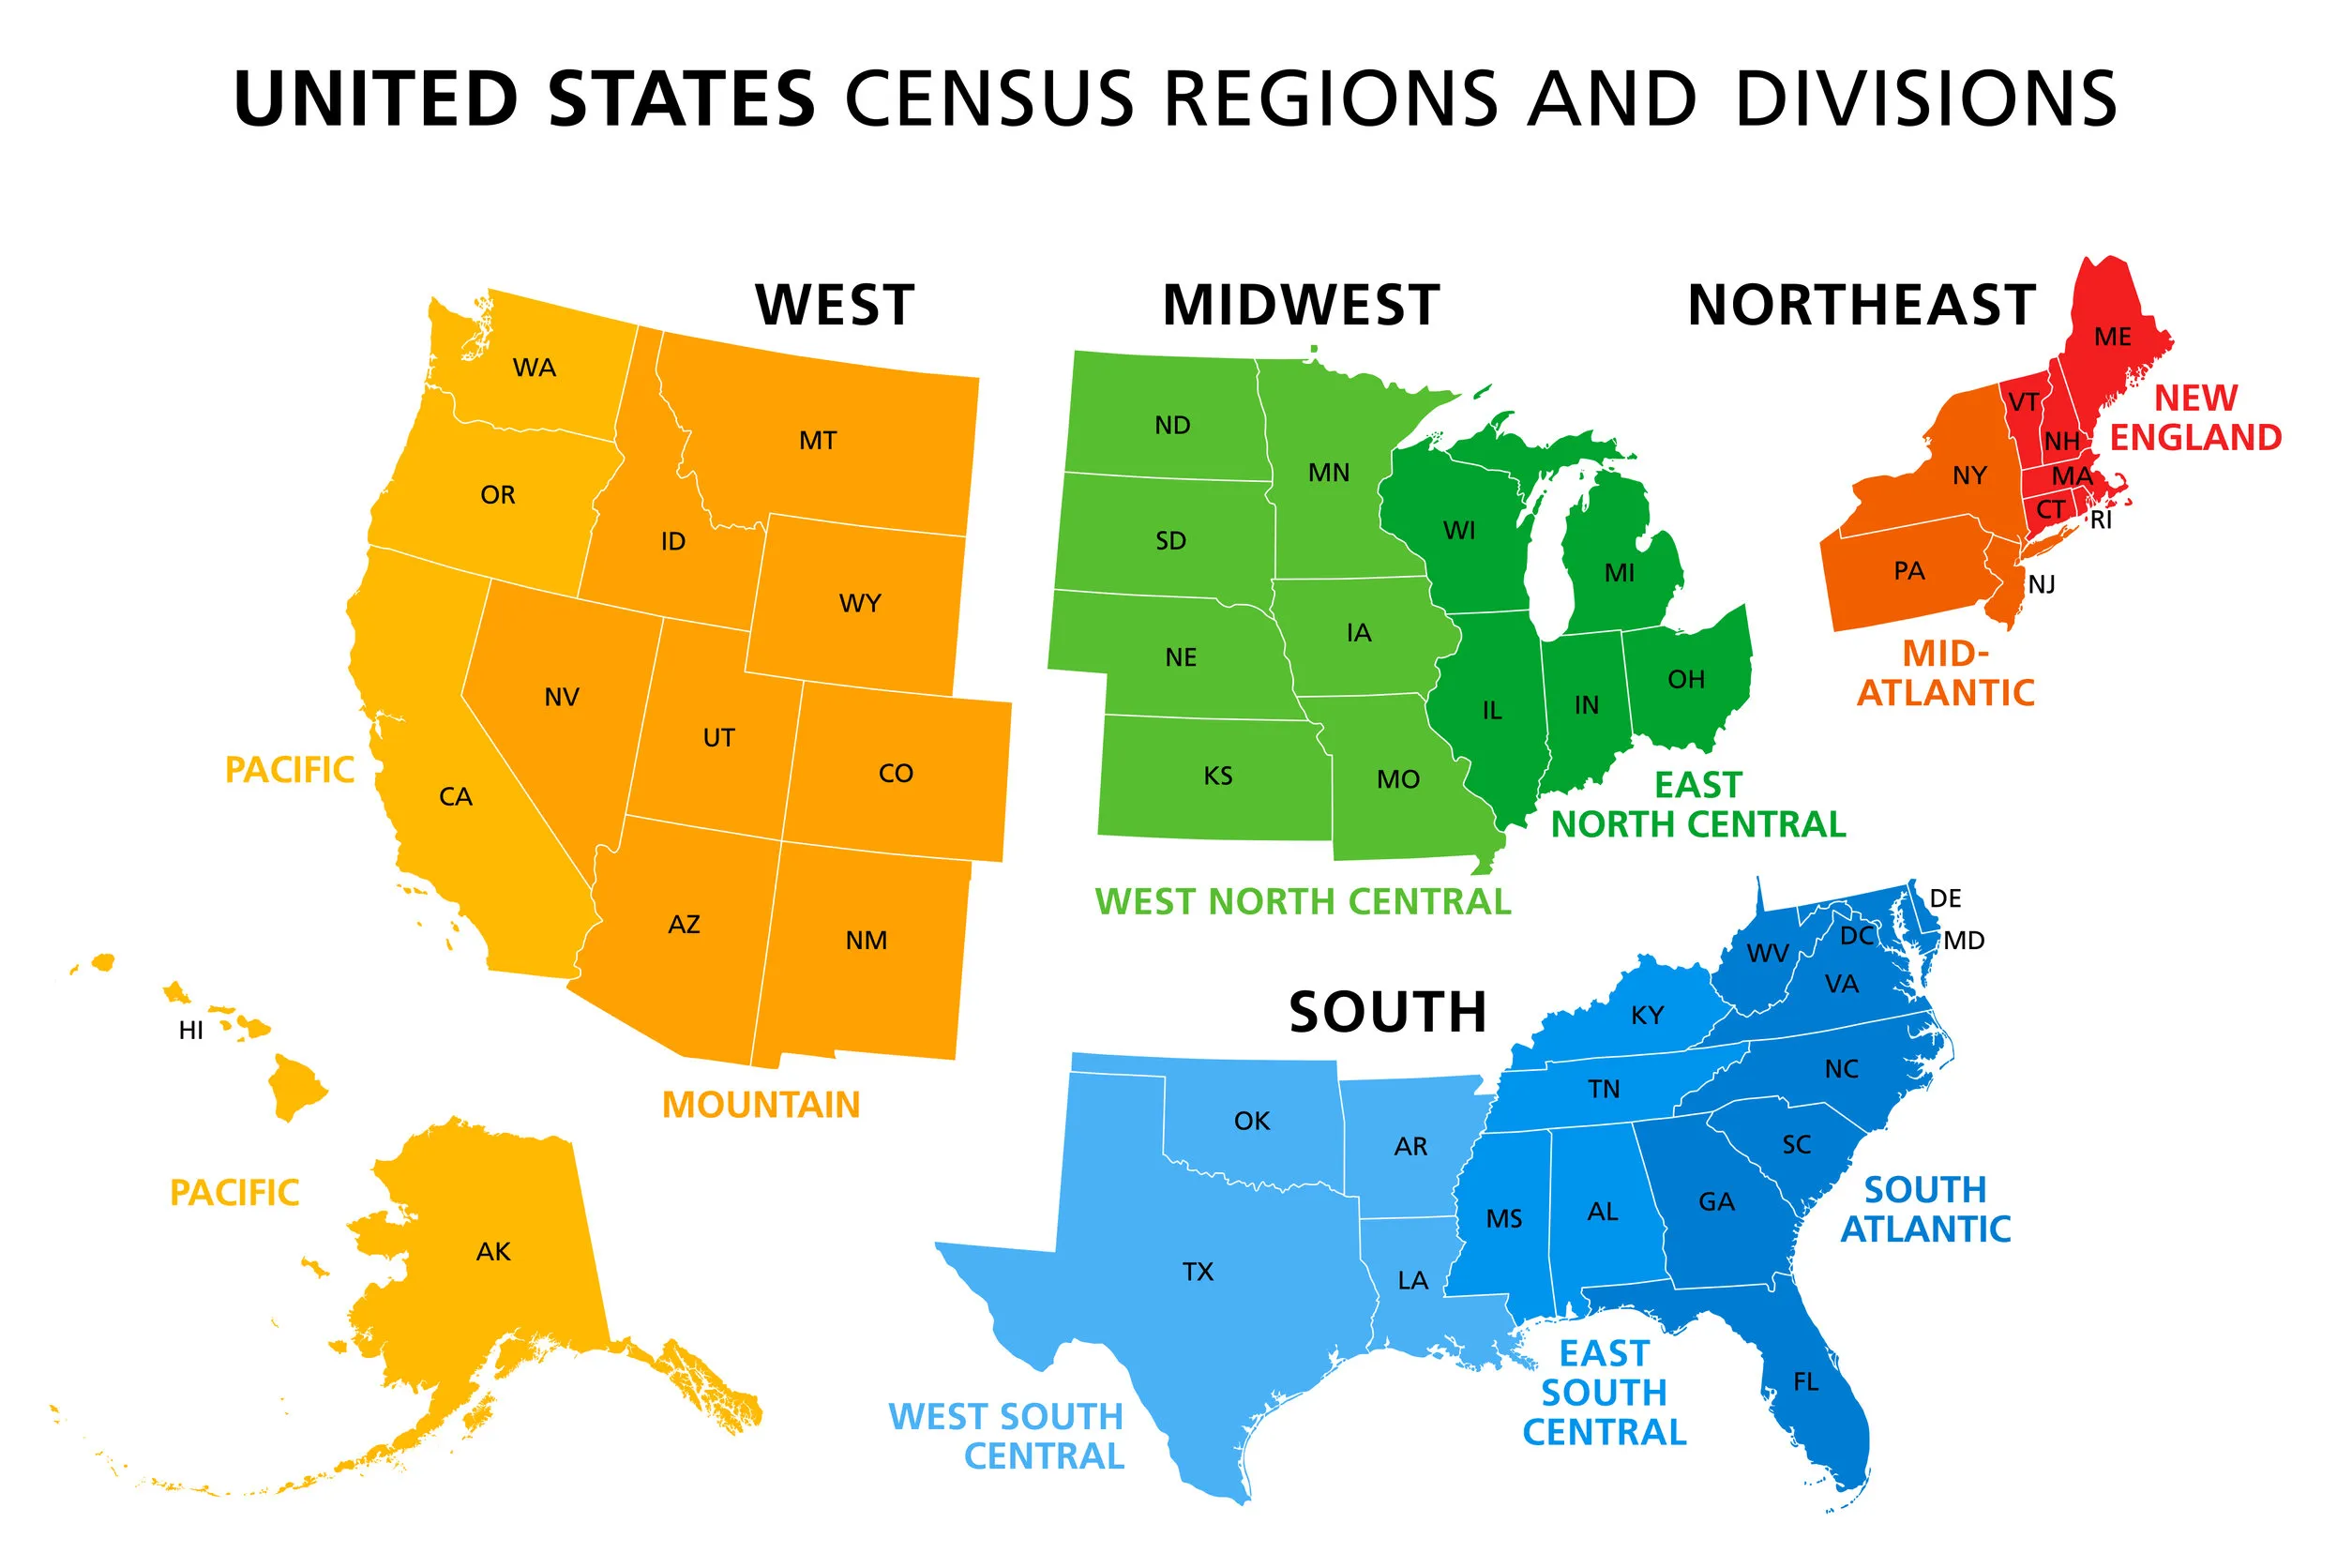
\includegraphics[scale=0.06]{us_regions.png}

\end{frame}

\begin{frame}{Linear regression with a categorical predictor}
What can we do? We can use \textcolor{blue}{dummy variables}\dots

\vspace{0.3cm}

\textcolor{blue}{Dummy variables}: The set of \textit{binary} variables created by re-writing (or re-coding) a multilevel categorical variable  

\vspace{0.3cm}

Example: Suppose we have a multilevel categorical variable for US region, with values West, Midwest, South, and Northeast

\vspace{0.3cm}

We create the new variables:
\begin{itemize}
	\item Midwest: \textit{Midwest} = 1 if \textit{region} = \textit{Midwest}, and 0 otherwise
	\item South: \textit{South} = 1 if \textit{region} = \textit{South}, and 0 otherwise
	\item Northeast: \textit{Northeast} = 1 if \textit{region} = \textit{Northeast}, and 0 otherwise
\end{itemize} \pause

\vspace{0.1cm}

\textcolor{blue}{Question:} We didn't make a dummy variable for West. Why not? \pause

\textcolor{blue}{Answer:} If all other dummy variables (Midwest, South, and Northeast) are 0, then the region must be West! In this case, West is referred to as a \textcolor{blue}{reference group}.
\end{frame} 

\begin{frame}{Linear regression with a categorical predictor}
Writing out our regression model for this example, we have
$$
E[\text{Outcome} \mid \text{Region}] = \beta_0 + \beta_1 \times \text{Midwest} + \beta_2 \times \text{South} + \beta_3 \times \text{Northeast}
$$

Note that we have more than just an intercept and slope coefficient here (making our way towards multiple linear regression!)

\vspace{0.3cm}

\textcolor{blue}{Question}: How do we interpret the coefficients $\beta_0$, $\beta_1$, $\beta_2$, $\beta_3$? \pause

\vspace{0.3cm}

$\beta_0$: average outcome among those in the Western region

$$
E[\text{Outcome} \mid \text{Region = West}] = \beta_0 + \beta_1 \times 0 + \beta_2 \times 0 + \beta_3 \times 0
$$


\end{frame}

\begin{frame}{Linear regression with a categorical predictor}
Writing out our regression model for this example, we have
$$
E[\text{Outcome} \mid \text{Region}] = \beta_0 + \beta_1 \times \text{Midwest} + \beta_2 \times \text{South} + \beta_3 \times \text{Northeast}
$$

Note that we have more than just an intercept and slope coefficient here (making our way towards multiple linear regression!)

\vspace{0.3cm}

\textcolor{blue}{Question}: How do we interpret the coefficients $\beta_0$, $\beta_1$, $\beta_2$, $\beta_3$?

\vspace{0.3cm}

$\beta_1$: difference in average outcome between groups in the Western region and Midwest region

\begin{align*}
E[&\text{Outcome} \mid  \text{Region = Midwest}] - E[\text{Outcome} \mid \text{Region = West}] \\
& = [\beta_0 + \beta_1 \times 1 + \beta_2 \times 0 + \beta_3 \times 0] - [\beta_0 + \beta_1 \times 0 + \beta_2 \times 0 + \beta_3 \times 0] \\
& = \beta_0 + \beta_1 - \beta_0 \\
& = \beta_1
\end{align*}


\end{frame}

\begin{frame}{Linear regression with a categorical predictor}
Writing out our regression model for this example, we have
$$
E[\text{Outcome} \mid \text{Region}] = \beta_0 + \beta_1 \times \text{Midwest} + \beta_2 \times \text{South} + \beta_3 \times \text{Northeast}
$$

Note that we have more than just an intercept and slope coefficient here (making our way towards multiple linear regression!)

\vspace{0.3cm}

\textcolor{blue}{Question}: How do we interpret the coefficients $\beta_0$, $\beta_1$, $\beta_2$, $\beta_3$?

\vspace{0.3cm}

$\beta_2$: difference in average outcome between groups in the Western region and Southern region

\begin{align*}
E[&\text{Outcome} \mid  \text{Region = South}] - E[\text{Outcome} \mid \text{Region = West}] \\
& = [\beta_0 + \beta_1 \times 0 + \beta_2 \times 1 + \beta_3 \times 0] - [\beta_0 + \beta_1 \times 0 + \beta_2 \times 0 + \beta_3 \times 0] \\
& = \beta_0 + \beta_2 - \beta_0 \\
& = \beta_2
\end{align*}


\end{frame}

\begin{frame}{Linear regression with a categorical predictor}
Writing out our regression model for this example, we have
$$
E[\text{Outcome} \mid \text{Region}] = \beta_0 + \beta_1 \times \text{Midwest} + \beta_2 \times \text{South} + \beta_3 \times \text{Northeast}
$$

Note that we have more than just an intercept and slope coefficient here (making our way towards multiple linear regression!)

\vspace{0.3cm}

\textcolor{blue}{Question}: How do we interpret the coefficients $\beta_0$, $\beta_1$, $\beta_2$, $\beta_3$?

\vspace{0.3cm}

$\beta_3$: difference in average outcome between groups in the Western region and Northeastern region

\begin{align*}
E[&\text{Outcome} \mid  \text{Region = Northeast}] - E[\text{Outcome} \mid \text{Region = West}] \\
& = [\beta_0 + \beta_1 \times 0 + \beta_2 \times 0 + \beta_3 \times 1] - [\beta_0 + \beta_1 \times 0 + \beta_2 \times 0 + \beta_3 \times 0] \\
& = \beta_0 + \beta_3 - \beta_0 \\
& = \beta_3
\end{align*}

\end{frame}

\begin{frame}{Linear regression with a categorical predictor: summary}
Our example:
$$
E[\text{Outcome} \mid  \text{Region = Northeast}] - E[\text{Outcome} \mid \text{Region = West}] 
$$

\begin{itemize}
	\item If we have $k$ categories, we create $k - 1$ \textcolor{blue}{dummy variables}, with the $k$th category being the \textcolor{blue}{reference group} captured in the intercept
	\item \texttt{R} automatically creates these dummy variables for you for multilevel categorical variables, as you'll see on your homework
\end{itemize}

\vspace{0.3cm}

Hypothesis testing: If we want to test whether our outcome is associated with a multilevel categorical variable, we need to test if \textit{all} coefficients for the dummy variables (in this example, $\beta_1, \beta_2, \beta_3$) are equal to zero.

\end{frame}

\begin{frame}{Linear regression with a categorical predictor: Example in \texttt{R}}
Suppose we're interested in whether birthweight is associated with race, in our births dataset. We can fit a linear regression model as before with simple linear regression, and look at the output\dots

\vspace{0.3cm}

\centering

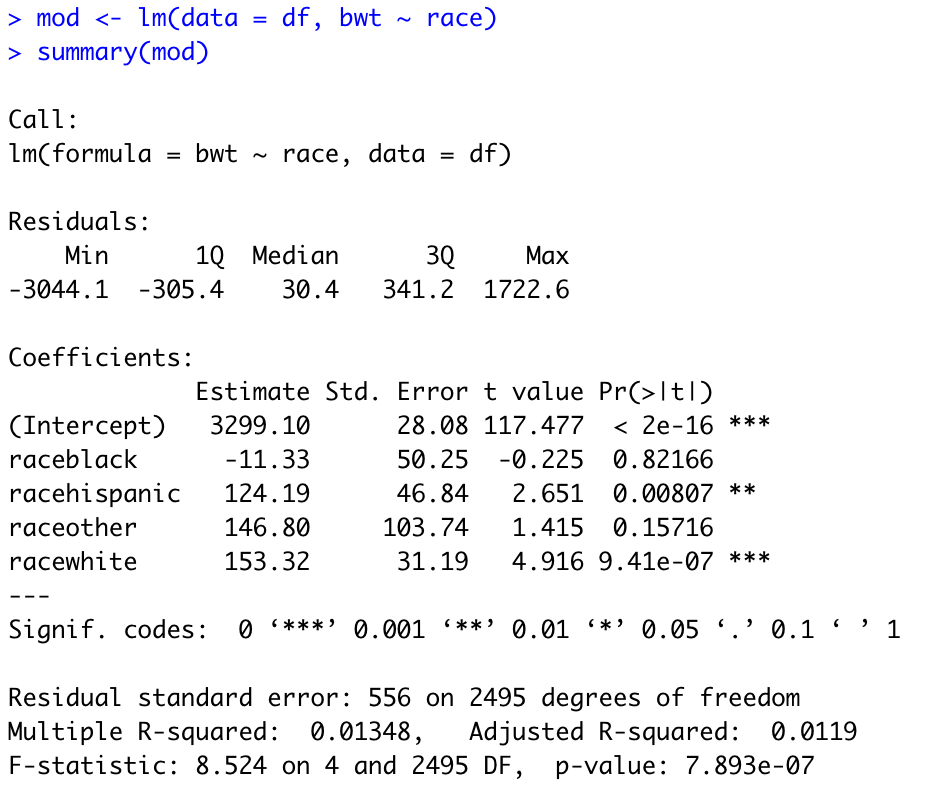
\includegraphics[scale=0.4]{multilevel_cat_lm.png}

\end{frame}

\begin{frame}{Linear regression with a categorical predictor: Example in \texttt{R}}

\begin{figure}
	\centering 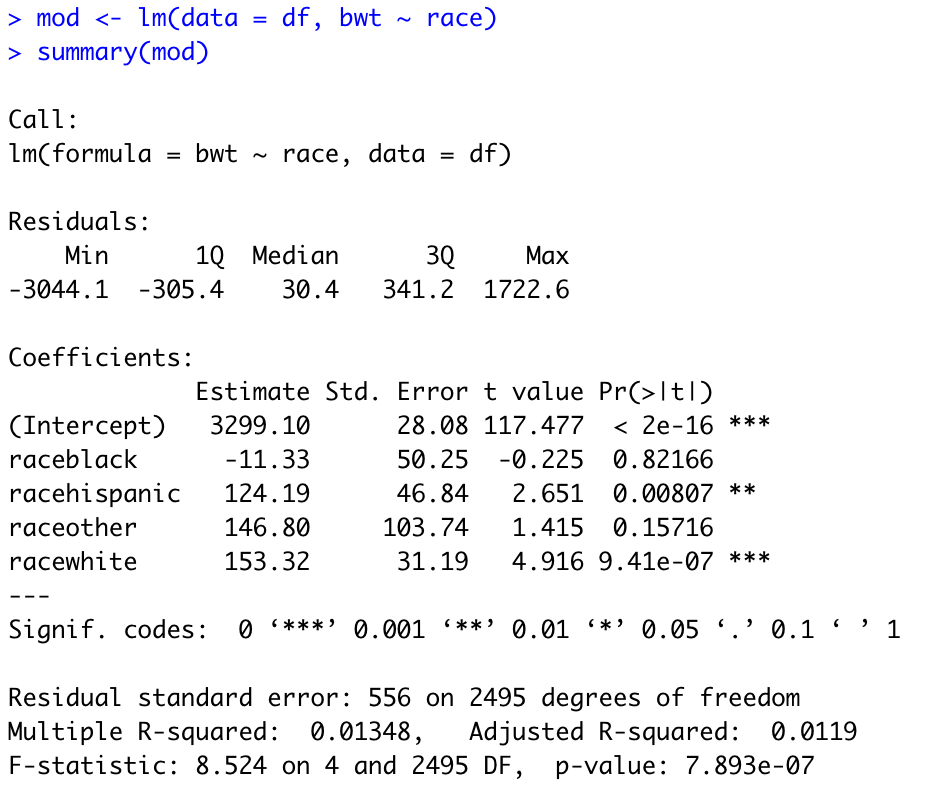
\includegraphics[scale=0.3]{multilevel_cat_lm.png}
\end{figure}

\vspace{0.1cm}

A couple things to notice:


\end{frame}

\begin{frame}{Linear regression with a categorical predictor: Example in \texttt{R}}

\begin{figure}
	\centering 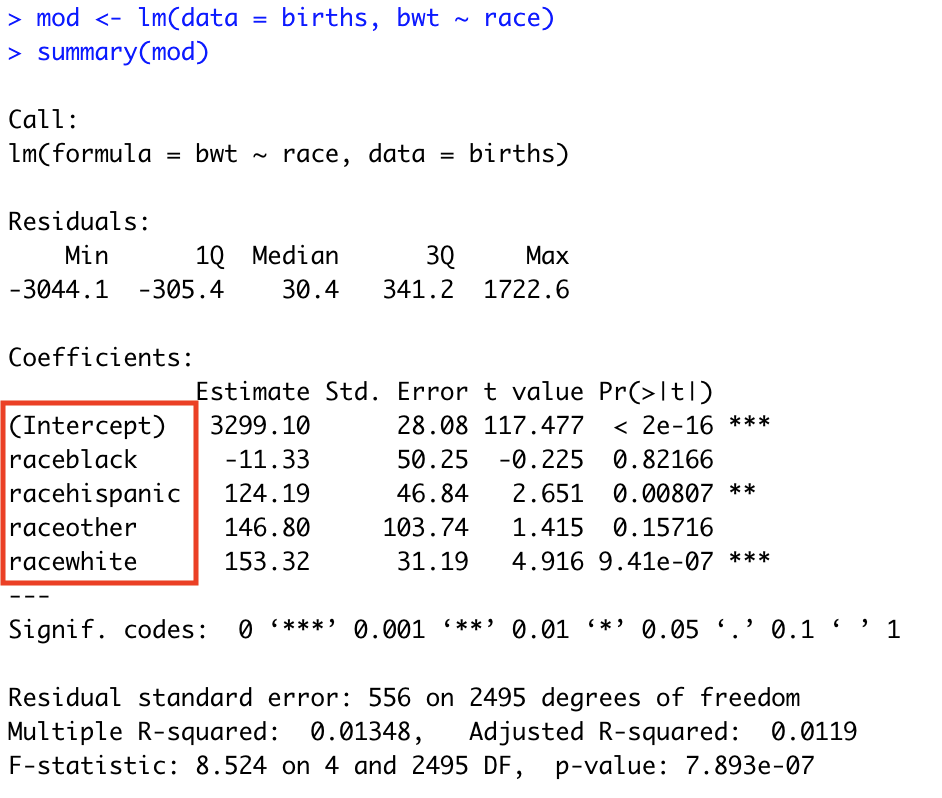
\includegraphics[scale=0.3]{multilevel_cat_lm2.png}
\end{figure}

\vspace{0.1cm}

A couple things to notice:
\begin{itemize}
	\item \texttt{R} has created dummy variables for us! The reference group by default will be the first category alphabetically (in this case, ``asian").
\end{itemize}

\end{frame}

\begin{frame}{Linear regression with a categorical predictor: Example in \texttt{R}}

\begin{figure}
	\centering 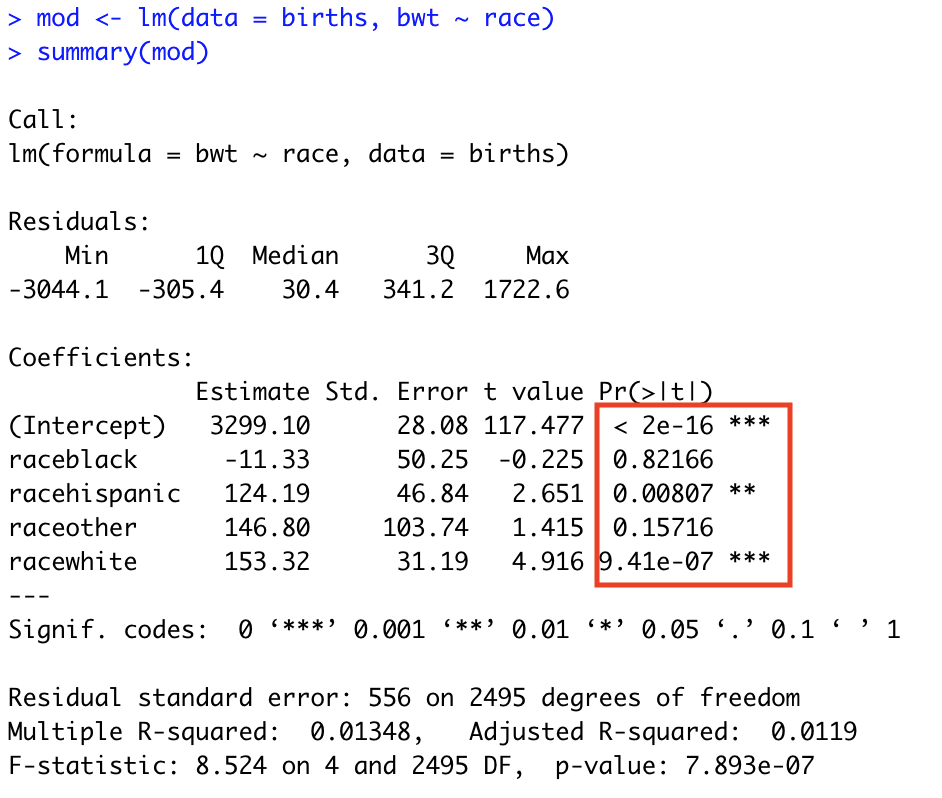
\includegraphics[scale=0.3]{multilevel_cat_lm3.png}
\end{figure}

\vspace{0.1cm}

A couple things to notice:
\begin{itemize}
	\item We have multiple p-values! But which p-value is the one associated with our hypothesis test? Let's write it down\dots
\end{itemize}

\end{frame}

\begin{frame}{Linear regression with a categorical predictor: Example in \texttt{R}}
We're interested in whether birthweight is associated with race, in our births dataset. Our regression model has the form:
$$
E[\text{bwt} \mid \text{race}] = \beta_0 + \beta_1 \times \text{black} + \beta_2 \times \text{hispanic} + \beta_3 \times \text{other} + \beta_4 \times \text{white}
$$ \pause

Our null hypthesis (in words) is that there is no association between race and birthweight. This would mean that \textcolor{blue}{all dummy variables for race} are \textit{simultaneously} equal to zero. \pause In math:

\vspace{0.3cm}

\begin{itemize}
	\item $H_0$: $\beta_1 = \beta_2 = \beta_3 = 0$
	\item $H_1$: \textit{at least one} of $\beta_1, \beta_2, \beta_3$ is not equal to $0$
\end{itemize} \pause

\vspace{0.3cm}

How do we do this in \texttt{R}?

\end{frame}

\begin{frame}{Linear regression with a categorical predictor: Example in \texttt{R}}
In \texttt{R}, we create two linear regression models: one with the race variable and an intercept, and one with only an intercept. We then use the \texttt{anova} function to test whether the race variable as a whole is significantly associated with birthweight.

\vspace{0.3cm}

\texttt{mod1 <- lm(data = df, bwt} $\sim$ \texttt{1) \\
	mod2 <- lm(data = df, bwt} $\sim$ \texttt{race) \\
	anova(mod1, mod2)} \pause

\vspace{0.3cm}

Details:
\begin{itemize}
	\item \texttt{mod1} is the model with only an intercept (specified with the $1$ on the right hand side of the tilde)
	\item Inside of the \texttt{anova} function, we put the ``smaller" model first (in this case, the model without the race covariate)
\end{itemize}
\end{frame}

\begin{frame}{Linear regression with a categorical predictor: Example in \texttt{R}}

Our output from the \texttt{anova} function:

\vspace{0.3cm}

\begin{figure}
	\centering 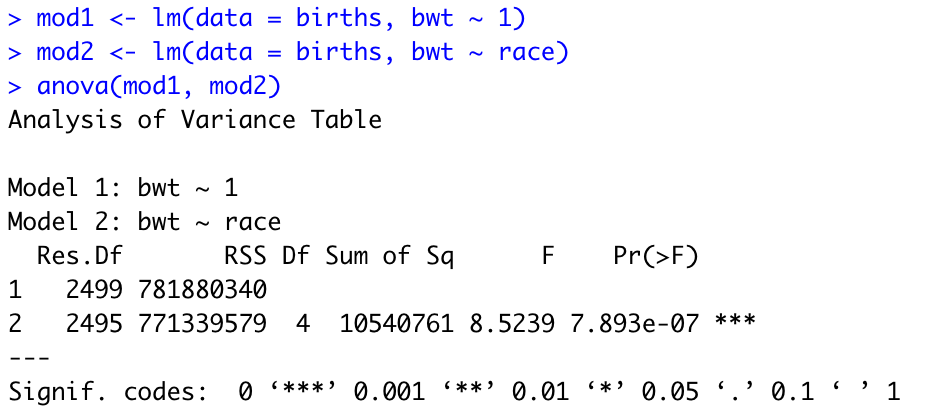
\includegraphics[scale=0.4]{anova_race.png}
\end{figure}

\end{frame}

\begin{frame}{Linear regression with a categorical predictor: Example in \texttt{R}}
Our output from the \texttt{anova} function:

\vspace{0.3cm}

\begin{figure}
	\centering 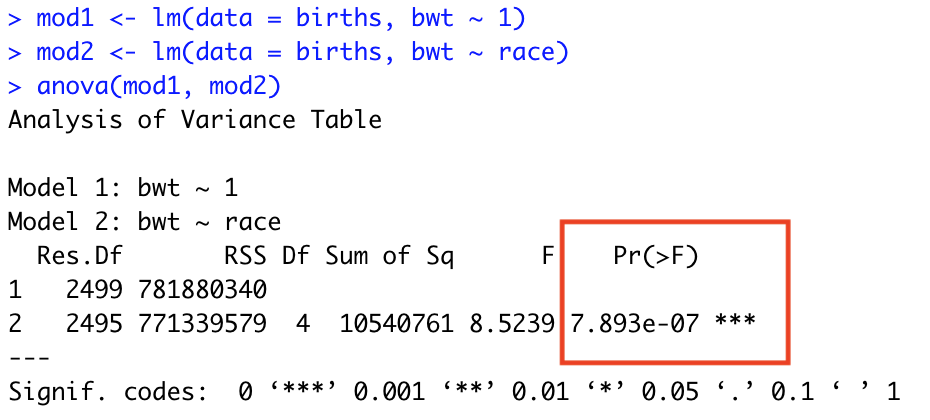
\includegraphics[scale=0.4]{anova_race2.png}
\end{figure}

\vspace{0.3cm}

\textit{This} is the p-value for our hypothesis test. \textit{Not} the individual p-values from our linear regression output. \pause

\vspace{0.3cm}



\includegraphics[scale=0.01]{chilipepper.png} \tiny You might notice that the p-value here corresponds to an F statistic, as opposed to a $t$ statistic as with hypothesis tests for single coefficients (e.g., $\beta_1 = 0$ vs. $\beta_1 \neq 0$). The key here is that F tests allow us to test for multiple coefficients being equal to $0$ at once. If you're interested in mathematical details, please ask us!

\end{frame}

\begin{frame}{Linear regression with a categorical predictor: Example in \texttt{R}}
Key Takeaway(s):
\vspace{0.3cm}

\begin{itemize}
	\item The individual p-values for separate categories of a multilevel categorical variable \textit{do not} correspond to the hypothesis test for whether the variable is associatied with the outcome
	\item We use the \texttt{anova} function in \texttt{R} to get p-values that correspond to hypothesis tests where the null hypothesis involves setting \textit{more than one} coefficient equal to zero
\end{itemize} \pause

\vspace{0.3cm}

What does this example have to do with multiple linear regression? 

\vspace{0.3cm}

Multiple linear regression involves having \textit{multiple} predictors in your model. Multilevel categorical variables are a preview of multiple linear regression, as they can be framed as multiple dummy variables! \pause

\vspace{0.2cm}

\tiny *note that the polynomial transformation also involved multiple predictors in our model, so you've now had two previews of multiple linear regression

\end{frame}

\subsection{Graphical examples}

\begin{frame}{Multiple linear regression: Motivation}
So far, we have considered the relationship between the outcome $Y$ and a single covariate/predictor $X$. Some terminology we'll use:

\vspace{0.3cm}

\textcolor{blue}{Predictor of interest}: the covariate whose relationship to the outcome corresponds to our primary scientific/statistical question \pause

\vspace{0.3cm}

In everything we've done so far $X$ has been our predictor of interest, but it also been our \textit{only} predictor. However, there may be other variables that \textit{influence} the association between our predictor of interest and the outcome, by:

\vspace{0.3cm}

\begin{itemize}
	\item \textcolor{blue}{Confounding} the association
	\item \textcolor{blue}{Modifying} the association
	\item Providing information that \textcolor{blue}{reduces the variability} of our estimates
\end{itemize}

\end{frame}

\begin{frame}{Multiple linear regression: Motivation}
(1) Suppose we collect information on the variables $X_1$ and $Y$ for 50 individuals (plotted below). What is your best guess at the linear relationship between $X_1$ and $Y$ (i.e. how would you draw the simple linear regression line on this graph)?

\vspace{0.3cm}

\centering 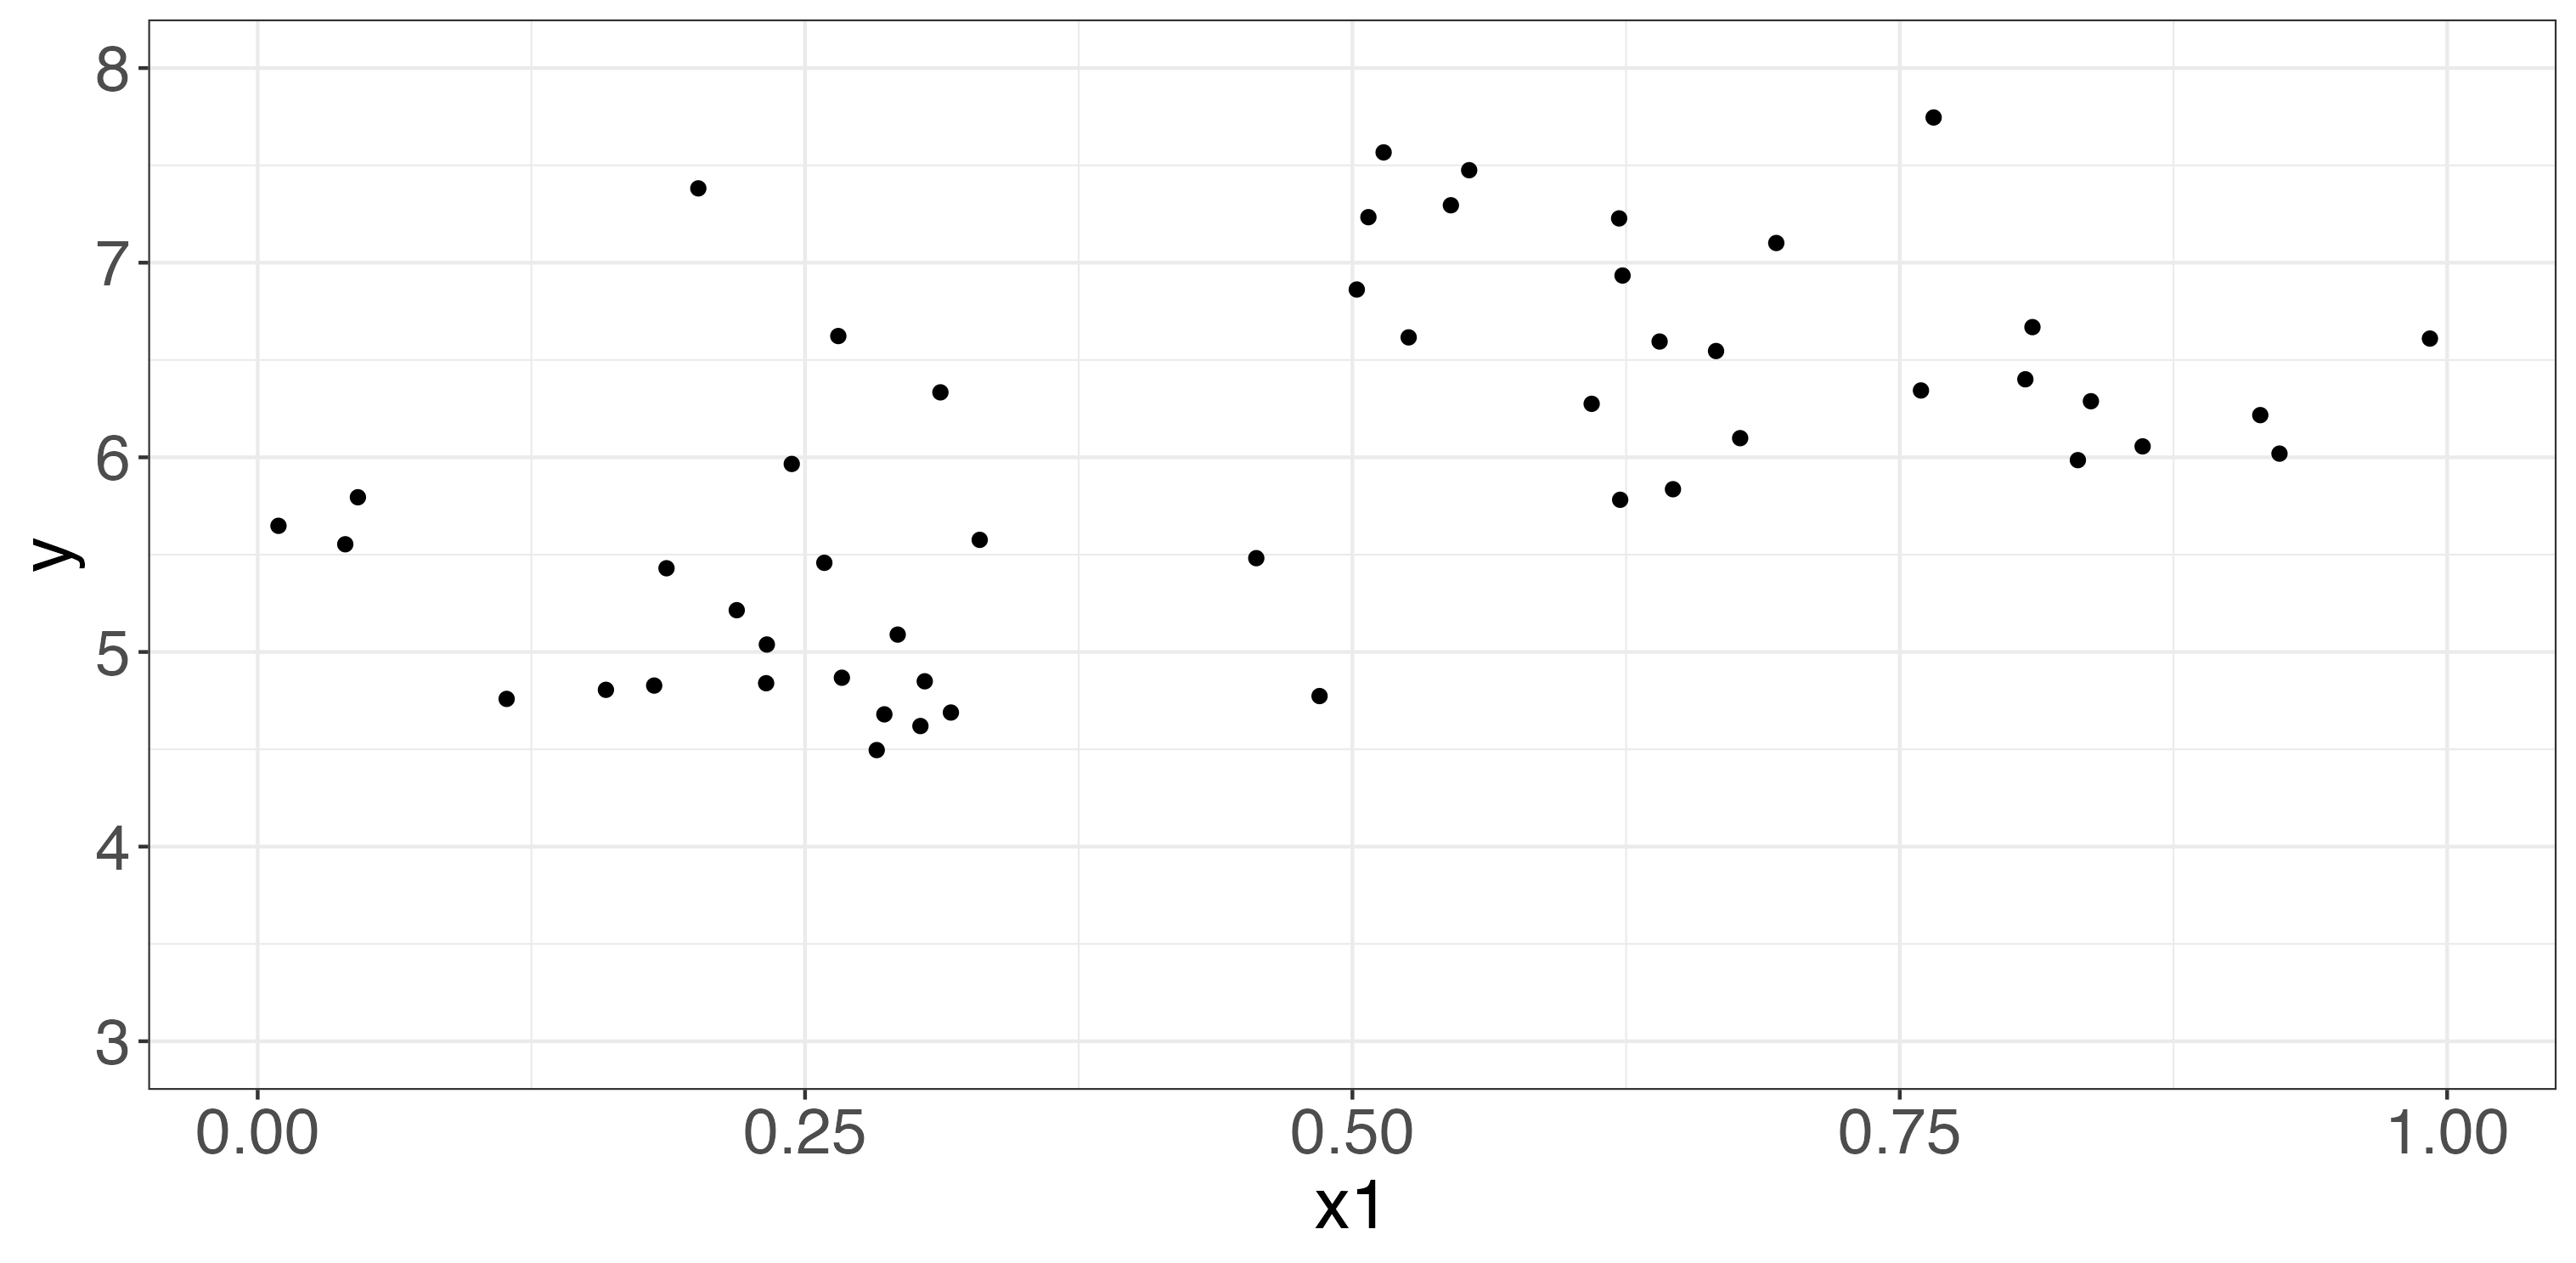
\includegraphics[scale=0.3]{multreg1.png}
\end{frame}

\begin{frame}{Multiple linear regression: Motivation}
(1) Suppose we collect information on the variables $X_1$ and $Y$ for 50 individuals (plotted below). What is your best guess at the linear relationship between $X_1$ and $Y$ (i.e. how would you draw the simple linear regression line on this graph)?

\vspace{0.3cm}

\centering 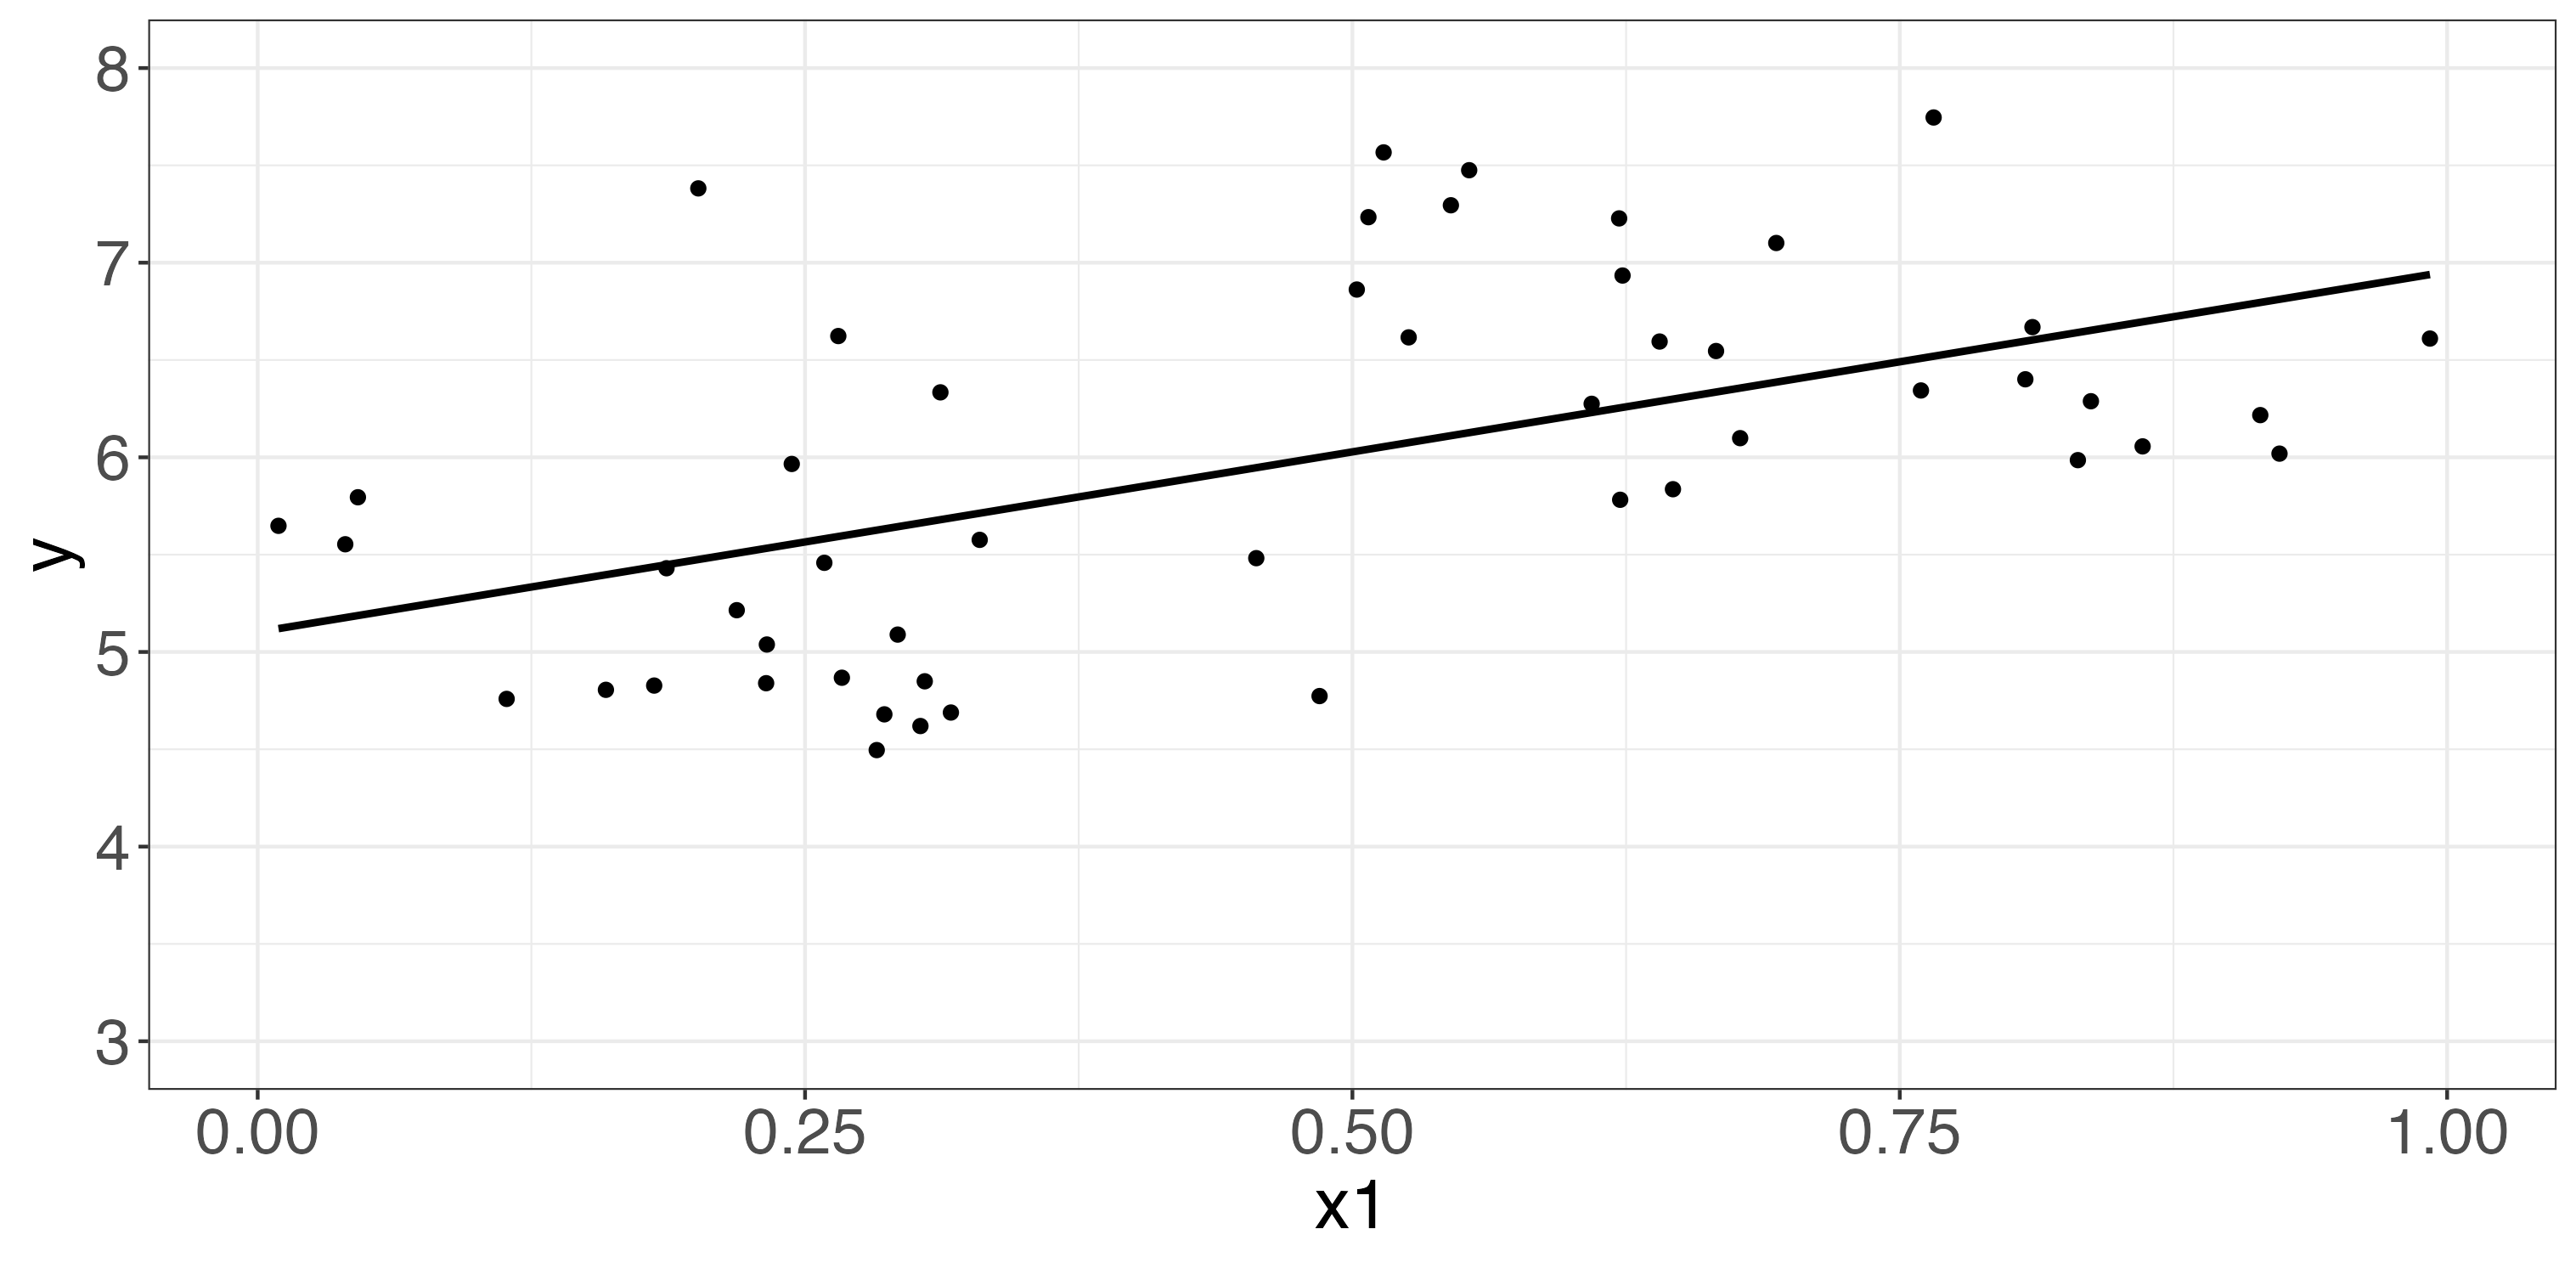
\includegraphics[scale=0.3]{multreg2.png}
\end{frame}

\begin{frame}{Multiple linear regression: Motivation}
(2) Suppose we also collected information on the binary variable $X_2$ for each individual. What is your best guess at the linear relationship between $X_1$ and $Y$, \textit{for each group} defined by the variable $X_2$? 

\vspace{0.3cm}

\centering 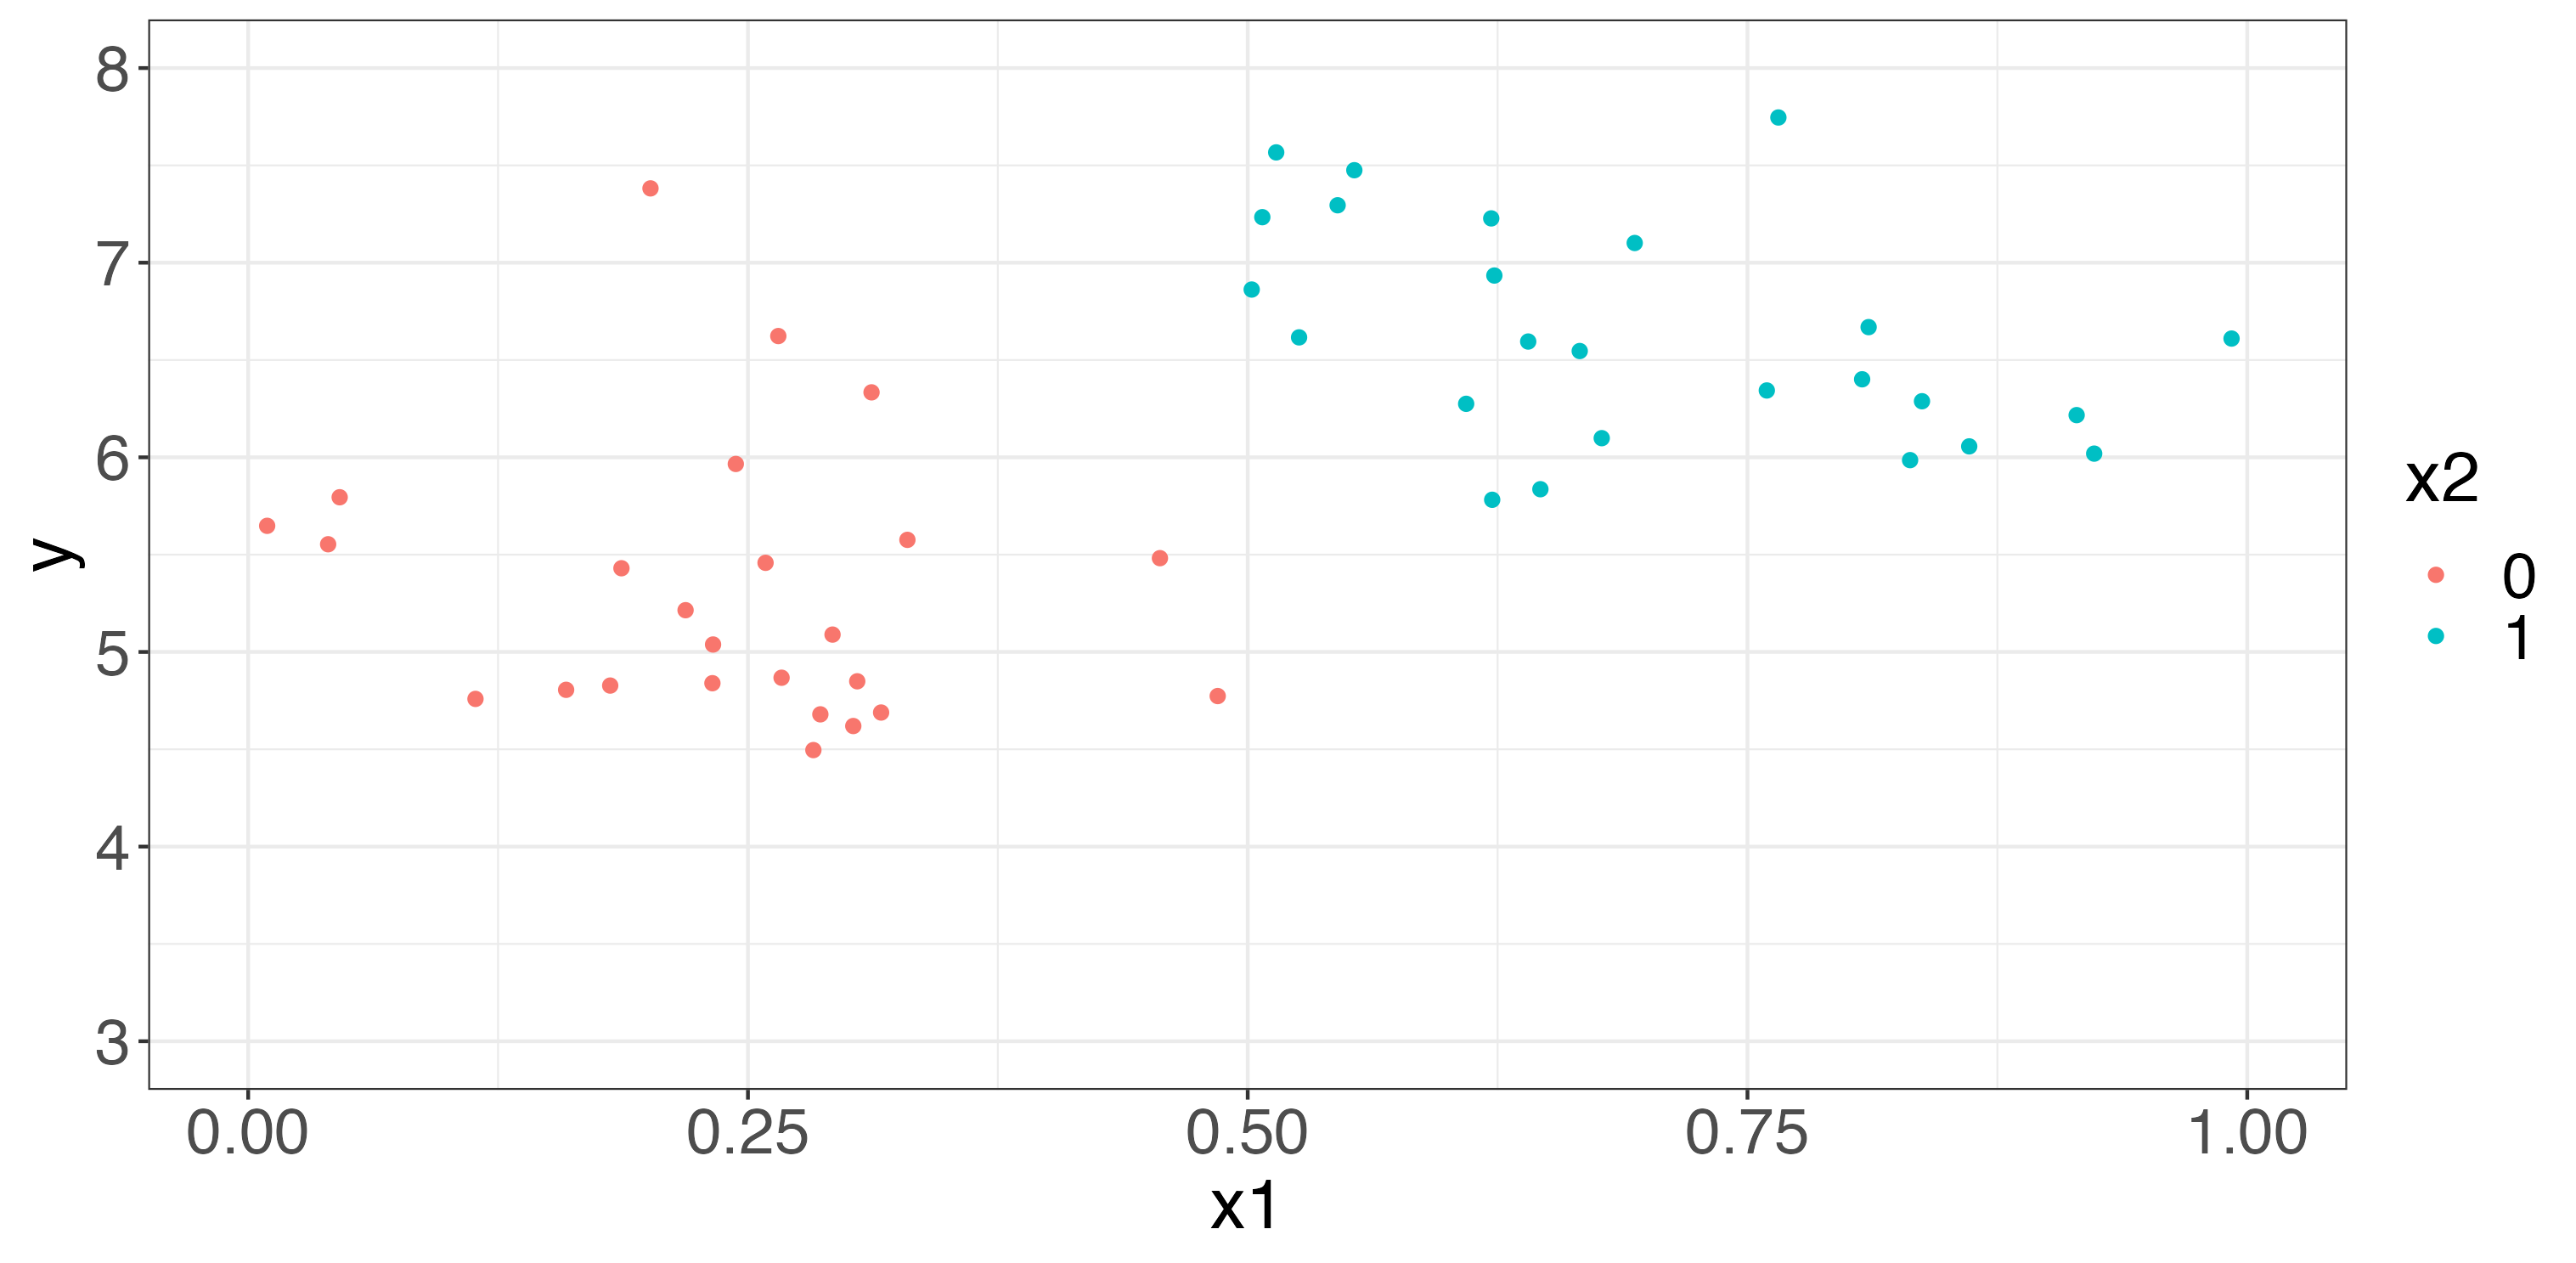
\includegraphics[scale=0.3]{multreg3.png}

\end{frame}

\begin{frame}{Multiple linear regression: Motivation}
(2) Suppose we also collected information on the binary variable $X_2$ for each individual. What is your best guess at the linear relationship between $X_1$ and $Y$, \textit{for each group} defined by the variable $X_2$? 

\vspace{0.3cm}

\centering 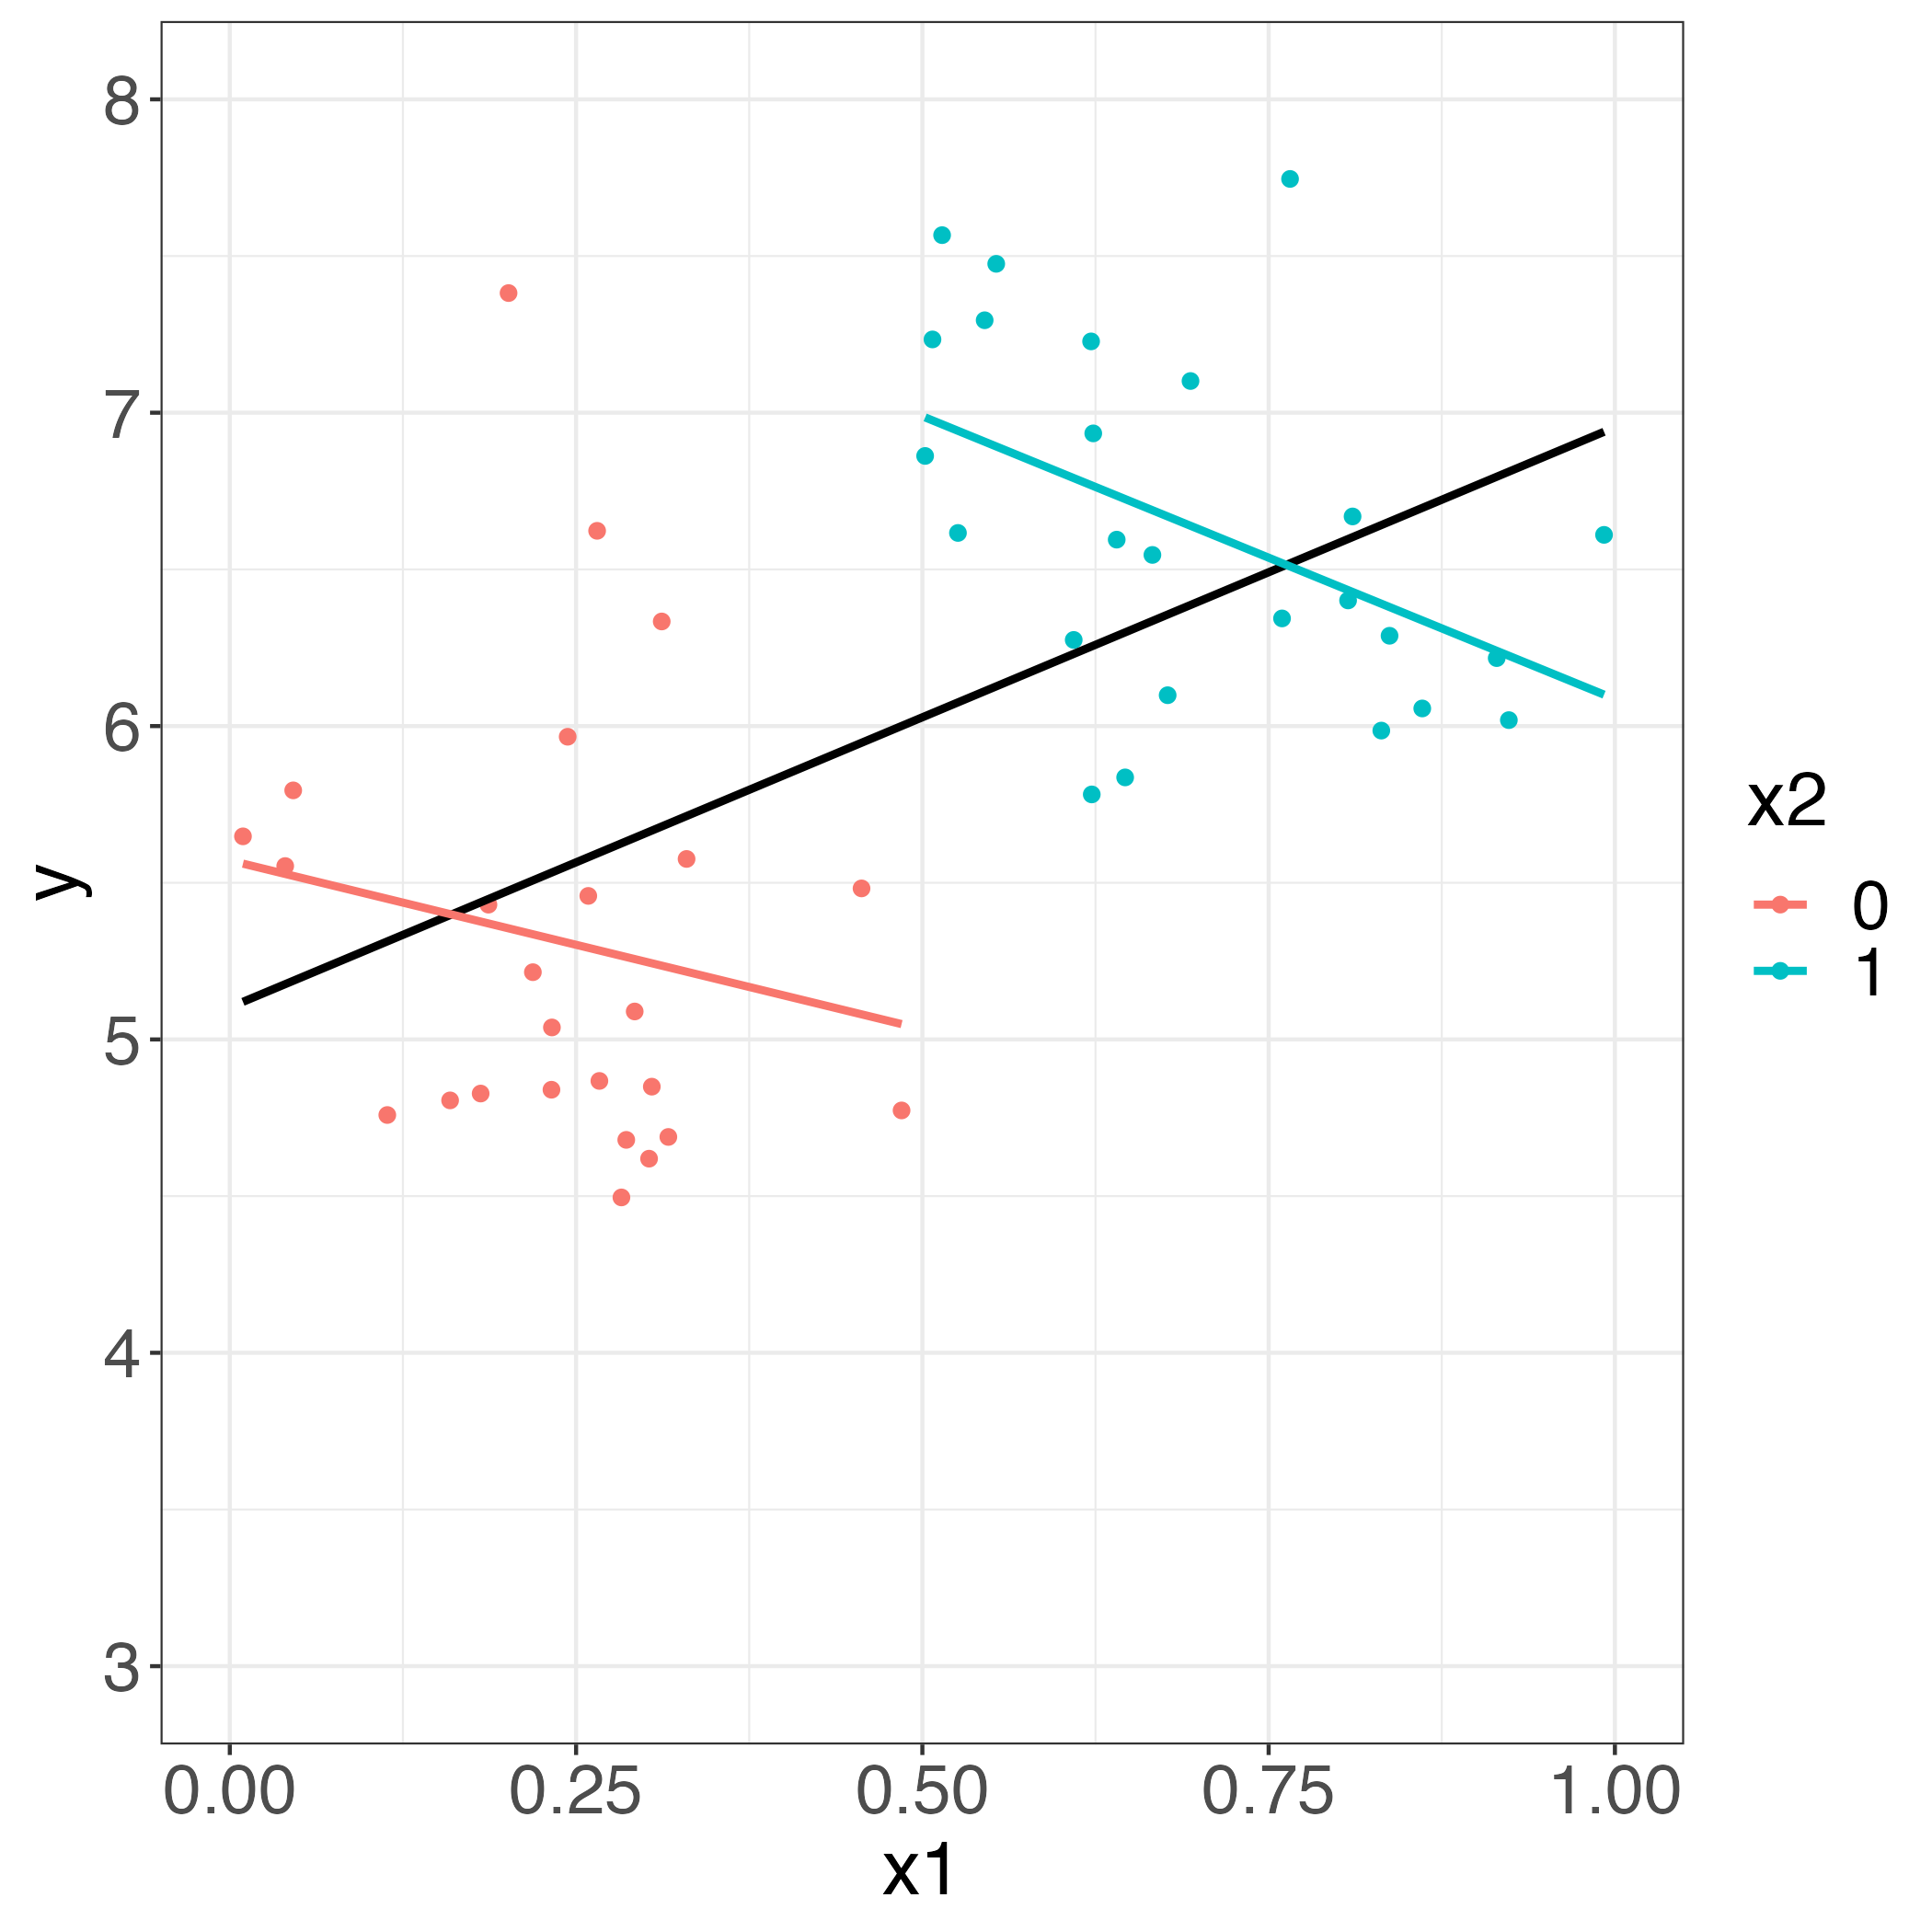
\includegraphics[scale=0.3]{multreg4.png}

\end{frame}

\begin{frame}{Multiple linear regression: Motivation}
\begin{figure}
	\centering 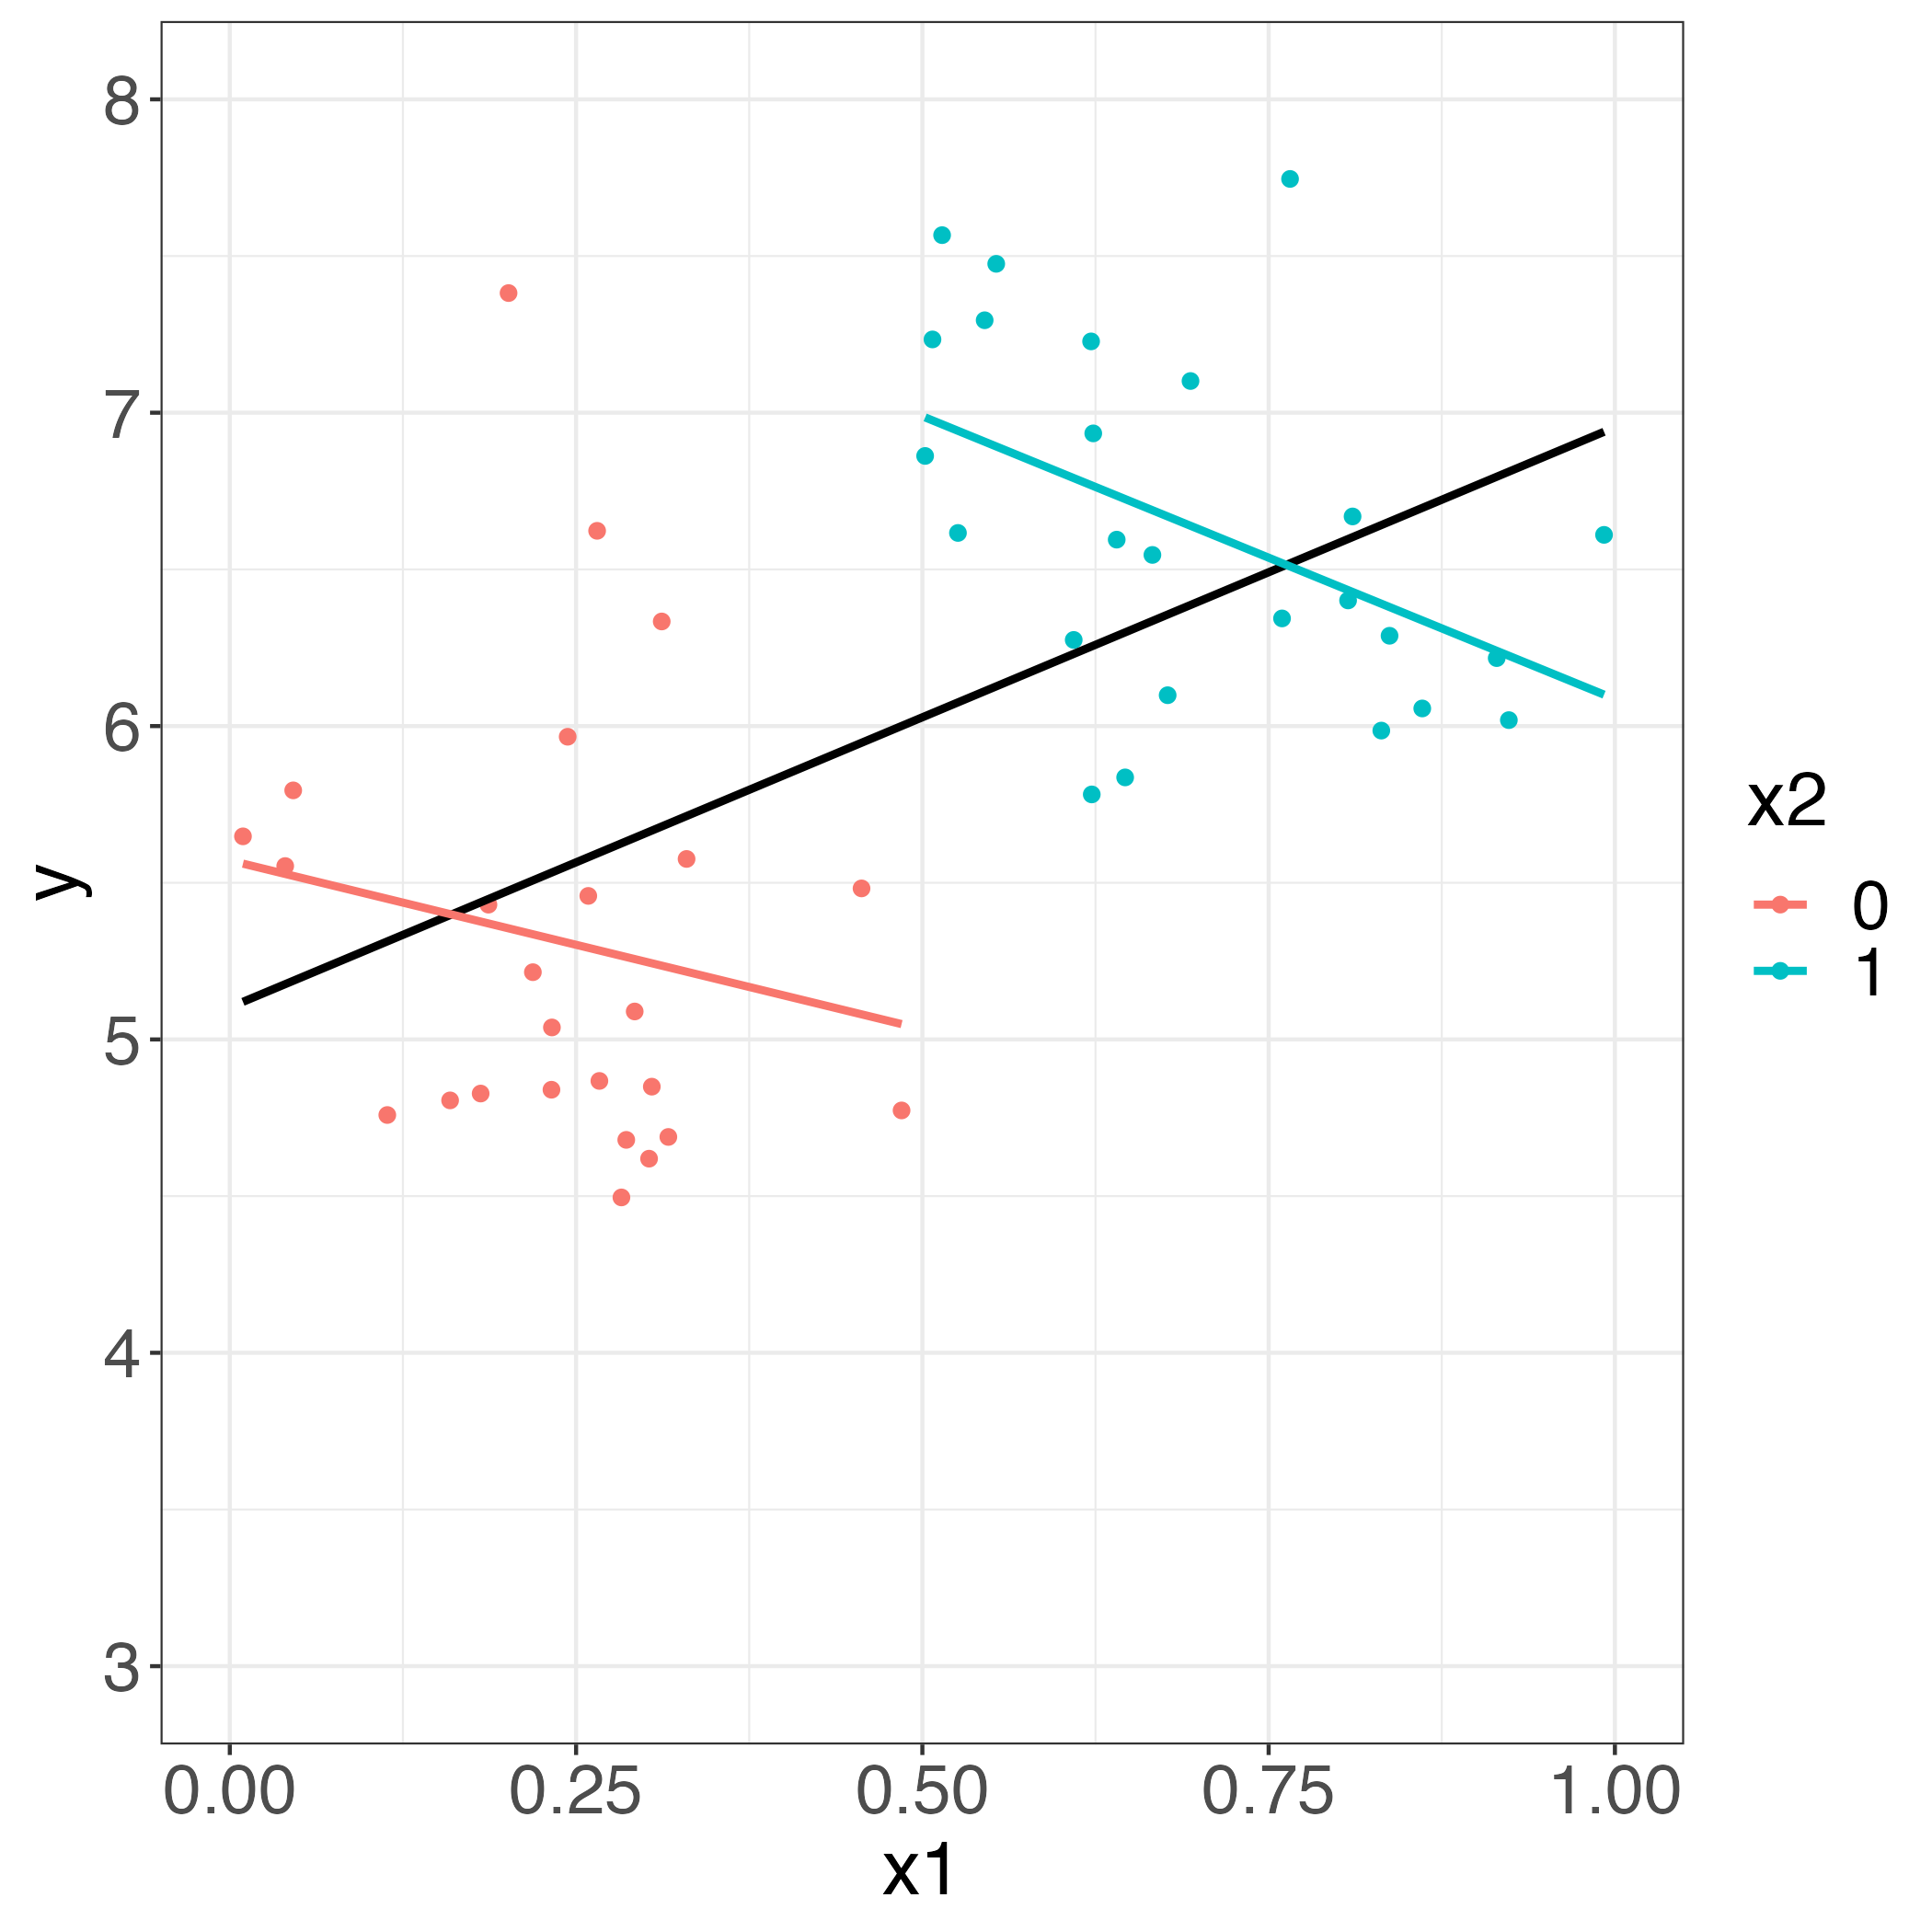
\includegraphics[scale=0.2]{multreg4.png}
\end{figure}

\vspace{0.1cm}

A couple things to note:

\begin{itemize}
	\item The best fitting line for the relationship between $X_1$ and $Y$ is different when we ignore $X_2$ vs. the best fitting lines for the relationship between $X_1$ and $Y$ for each group defined by $X_2$
	\item The lines we drew were in response to \textit{different} questions:
	\begin{enumerate}
		\item What is your best guess at the linear relationship between $X_1$ and $Y$?
		\item What is your best guess at the linear relationship between $X_1$ and $Y$, \textit{for each group} defined by the variable $X_2$? 
	\end{enumerate}
\end{itemize}

\end{frame}

\begin{frame}{Multiple linear regression: Motivation}
\begin{itemize}
	\item The best fitting line for the relationship between $X_1$ and $Y$ is different when we ignore $X_2$ vs. the best fitting lines for the relationship between $X_1$ and $Y$ for each group defined by $X_2$
	\item The lines we drew were in response to \textit{different} questions:
	\begin{enumerate}
		\item What is your best guess at the linear relationship between $X_1$ and $Y$?
		\item What is your best guess at the linear relationship between $X_1$ and $Y$, \textit{for each group} defined by the variable $X_2$? 
	\end{enumerate}
\end{itemize}

\vspace{0.3cm}

Multiple linear regression addresses questions like the latter, where we are interested in the relationship between an outcome and a \textcolor{blue}{predictor of interest}, while other variables may \textit{influence} the association between the predictor of interest and the outcome. \pause

\vspace{0.3cm}

\small *The graphical example on the previous slides is just one example of how the relationship between the outcome and predictor of interest may vary based on another variable! You may see more or less extreme differences in practice, and we'll show graphical examples for each of confounders, precision variables, and effect modifiers in the following section.
\end{frame}

\section{Adjusting for covariates}

\begin{frame}{Adjusting for covariates}
In simple linear regression, we modeled the expected value of $Y$ given a single predictor of interest $X_1$ as a linear function of the intercept and slope:

$$
E[Y \mid X_1] = \beta_0 + \beta_1 X_1
$$
\pause
In multiple linear regression, we'll start to add additional variables into our model. We will often call these additional variables \textcolor{blue}{covariates}. If we have a covariate $X_2$ that we want to include in our model, our regression form becomes

$$
E[Y \mid X_1, X_2] = \beta_0 + \beta_1 X_1 + \beta_2 X_2
$$

\end{frame}

\begin{frame}{Adjusting for covariates}
In simple linear regression, we modeled the expected value of $Y$ given a single predictor of interest $X_1$ as a linear function of the intercept and slope:

$$
E[Y \mid X_1] = \beta_0 + \beta_1 X_1
$$
In multiple linear regression, we'll start to add additional variables into our model. We will often call these additional variables \textcolor{blue}{covariates}. If we have a covariate $X_2$ that we want to include in our model, our regression form becomes

$$
E[Y \mid X_1, \textcolor{red}{X_2}] = \beta_0 + \beta_1 X_1 + \beta_2 X_2
$$

We've included \textcolor{red}{$X_2$} on the left-hand side of our equation, because our expected outcome now depends on both $X_1$ \textit{and} $X_2$.

\end{frame}

\begin{frame}{Adjusting for covariates}
In simple linear regression, we modeled the expected value of $Y$ given a single predictor of interest $X_1$ as a linear function of the intercept and slope:

$$
E[Y \mid X_1] = \beta_0 + \beta_1 X_1
$$
In multiple linear regression, we'll start to add additional variables into our model. We will often call these additional variables \textcolor{blue}{covariates}. If we have a covariate $X_2$ that we want to include in our model, our regression form becomes

$$
E[Y \mid X_1, X_2] = \beta_0 + \beta_1 X_1 + \color{red}{\beta_2 X_2}
$$

We've \textit{added} \textcolor{red}{$X_2$} to the right-hand side of our equation because with linear regression, our expected outcome is a \textit{linear combination} of predictors (this means we always add!). Note that $X_2$ also gets its own coefficient, $\beta_2$.

\end{frame}

\begin{frame}{Adjusting for covariates}
In simple linear regression, we modeled the expected value of $Y$ given a single predictor of interest $X_1$ as a linear function of the intercept and slope:

$$
E[Y \mid X_1] = \beta_0 + \beta_1 X_1
$$
In multiple linear regression, we'll start to add additional variables into our model. We will often call these additional variables \textcolor{blue}{covariates}. If we have a covariate $X_2$ that we want to include in our model, our regression form becomes

$$
E[Y \mid X_1, X_2] = \beta_0 + \beta_1 X_1 + \beta_2 X_2
$$

\textcolor{blue}{Question}: What if we want to include covariates $X_3, X_4, \dots, X_{100}$ in our model as well? What would the regression equation look like?
\end{frame}

\begin{frame}{Adjusting for covariates}
\textcolor{blue}{Question}: What if we want to additionally include covariates $X_3, X_4, \dots, X_{100}$ in our model as well? What would the regression equation look like?

\vspace{0.3cm}

\textcolor{blue}{Answer:} 

$$
E[Y \mid X_1, \dots, X_{100}] = \beta_0 + \beta_1 X_1 + \beta_2 X_2 + \dots + \beta_{100} X_{100}
$$

We include all of the covariates in our model on the left-hand side of the equation (after the conditional symbol, ``$|$"), and add all of the covariates to the right-hand side of the equation, each with their own coefficient.

\end{frame}

\begin{frame}{Adjusting for covariates}
In what situations would we want / need to include additional covariates in our regression model?

\vspace{0.3cm}

Scientific questions typically address one of three questions about the relationship between the predictor of interest and the outcome:

\vspace{0.3cm}

\begin{itemize}
	\item does the predictor of interest \textit{causally} effect the outcome?
	\item is there an association between the predictor of interest and the outcome?
	\item does the association (if it exists) differ in groups defined by an additional covariate?
\end{itemize} \pause

\vspace{0.3cm}

Depending on the \textcolor{blue}{study design} and \textcolor{blue}{scientific question}, we may need to include additional covariates in our model to answer these questions!

\end{frame}

\begin{frame}{Adjusting for covariates}
Throughout this section, we will consider three types of covariates that we may include in our multiple regression models:

\vspace{0.3cm}

\begin{enumerate}
	\item Confounders
	\item Precision variables
	\item Effect modifiers
\end{enumerate}

\vspace{0.3cm}

For each, we'll discuss their need for inclusion in a statistical model based on study design and scientific question. But first, we'll talk about \textcolor{blue}{causal diagrams}, which are a useful tool to help us visualize the potential relationships between variables.

\end{frame}

\subsection{Causal diagrams}

\begin{frame}{Causal diagrams}
\small \textcolor{blue}{This slide intentionally left blank for causal diagrams activity.}
\end{frame}

\subsection{Stratification}

\subsection{Confounders}

\subsection{Precision variables}

\subsection{Effect modifiers}



% motivator for multiple linear regression
% note that also had multiple coefficients with the polynomial transformation


\begin{frame}[c]
\centering \huge Any Questions?
\end{frame}

\end{document}